\chapter{Durchführung}
\label{cha:Durchführung}
Um ein Verständnis für den Laser, sowie das Verhalten bei verschiedenen Parametern zu erarbeiten werden verschiedene Messungen durchgeführt. Dafür wird zunächst der Laser mit den 
Steuer- und Messelementen verkabelt.

\section{Bestimmung des Schwellenstroms}
\label{sec:schwelle}

Um den Schwellenstrom zu messen, ab welchem der Laserbetrieb gewährleistet ist, wird der erwartete Laserstrahl auf eine Detektorkrate gesendet. Diese Detektorkarte reflektiert 
Infrarot so, dass es im optischen Bereich liegt. Mit einer CCD Kamera kann die Reflexion aufgenommen werden. Wird nun der Diodenstrom erhöht tritt ab einem Schwellenwert
Lasergranulation auf. Dies geschieht aufgrund von Beugungseffekten an einer unebenen Oberfläche. Charakteristisch zeigt sich dies durch ein fleckig geüunktetes Muster auf der Karte. 
Sobald dieses Muster auftritt ist der Schwellenstrom erreicht. 

\section{Aufnahme der Rubidiumfluoreszenz}
\label{sec:fluoreszenz}

Als nächstes wird der aktive Laser auf eine Rubidiumzelle gerichtet. Durch Relaxationsprozesse kann Fluoreszenz mit einer CCD Kamera aufgenommen werden. Wie in Abschnitt \ref{sec:rub}
beschrieben tritt dies allerdings nur für exakt definierte Wellenlängen auf. Die Wellenlänge kann durch Drehung des Gitters veriiert werden. Dies geschieht bis man Fluoreszenz beobachtet.

\section{Absorptionsspektrum von Rubidium}
\label{sec:abso_rub}

Um das Absorptionsspektrum von Rubidium zu messen wird ein Versuchaufbau nach Abbildung \ref{fig:Aufbau_rub} gebaut.

\begin{figure}
    \centering
    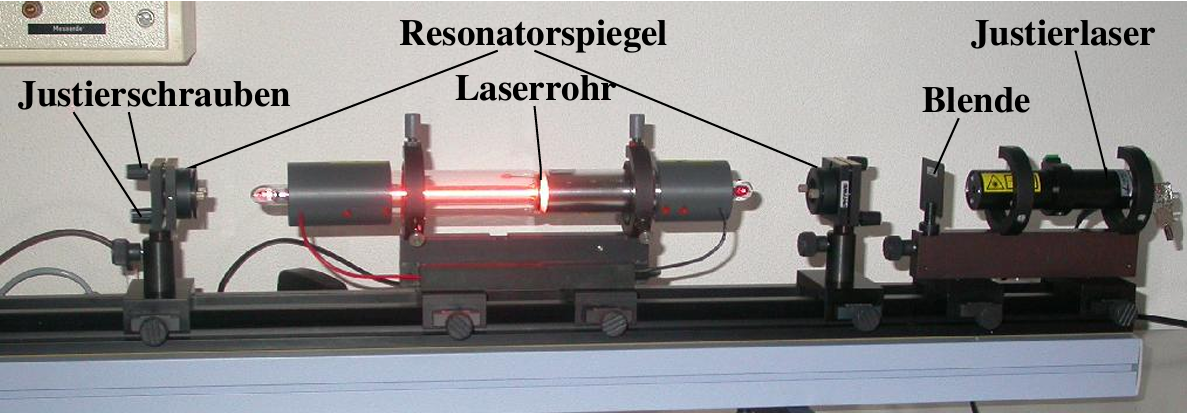
\includegraphics[width=\textwidth]{content/pics/Aufbau.png}
    \caption{Verwendeter Versuchsaufbau zur Bestimmung des Absorptionsspektrums der Rubidiumzelle \cite{diode_laser_spectroscopy}.}
    \label{fig:Aufbau_rub}
\end{figure}

Nun trifft der Laser zunächst auf einen 50/50 Strahlenteiler. An diesem wird der Strahl zum einen direkt in eine Photodiode gesendet und zum anderen durch die Rubidiumzelle auf einen 
weiteren Photodetektor gesendet. In einem Oszilloskop kann dann das Differenzsignal dargestellt werden. Dies ist nötig um Hintergrundrauschen zu minimieren und ein möglichst 
genaues Spektrum zu erhalten. 
